%\documentclass[handout]{beamer}
\documentclass{beamer}
\usepackage[ruled,linesnumbered]{algorithm2e}
\usepackage{natbib}
%\usepackage{enumitem}
\definecolor{vuborange}{rgb}{1.0,0.40,0.0}
\usetheme{Boadilla}
\usepackage{amsmath,amssymb}
\usepackage{booktabs}
\title{Efficiently Explaining CSPs with Unsatisfiable Subset Optimization}
\institute[shortinst]
{\inst{1} Vrije Universiteit Brussel, Belgium \\ % Your institution for the title page
	\inst{2} KULeuven, Belgium \\ % Your institution for the title page
	\href{mailto:emilio.gamba@vub.be}{\underline{emilio.gamba@vub.be}}, \href{mailto:bart.bogaerts@vub.be}{bart.bogaerts@vub.be}, \href{mailto:tias.guns@kuleuven.be}{tias.guns@kuleuven.be} % Your email address
}
\date{Siemens 08/03/2022}

\author{\underline{Emilio Gamba}\inst{1} \and  Bart Bogaerts\inst{1} \and   Tias Guns\inst{1,2}}

\newcommand\m[1]{\ensuremath{#1}\xspace}
\newcommand\allconstraints{\m{T_P}}
\newcommand\formula{\ensuremath{\m{F} }\xspace}
\newcommand\formulac{\ensuremath{\m{C} }\xspace}

\makeatletter
\setbeamertemplate{footline}
{
	\leavevmode%
	\hbox{%
		\begin{beamercolorbox}[wd=.2\paperwidth,ht=2.25ex,dp=1ex,center]{author in head/foot}%
			\usebeamerfont{author in head/foot}Emilio Gamba (VUB)
		\end{beamercolorbox}%
		\begin{beamercolorbox}[wd=.6\paperwidth,ht=2.25ex,dp=1ex,center]{title in head/foot}%
			\usebeamerfont{title in head/foot}Efficiently Explaining CSPs with Unsatisfiable Subset Optimization
		\end{beamercolorbox}%
		\begin{beamercolorbox}[wd=.2\paperwidth,ht=2.25ex,dp=1ex,right]{date in head/foot}%
			\usebeamerfont{date in head/foot}August 2021\hspace*{1em}
			\insertframenumber{} / \inserttotalframenumber\hspace*{2ex} 
	\end{beamercolorbox}}%
	\vskip0pt%
}
\makeatother

\begin{document}
	
	\begin{frame}
		\maketitle
	\end{frame}
	
	
	\begin{frame}
		\frametitle{Outline}
		
		\begin{enumerate}
			\item Context
			\begin{itemize}
				\item Boolean Satisfiability \pause
			\end{itemize}
			\item Goal
			\begin{itemize}
				\item Explaining \textbf{SAT} problems: Generate  a sequence of \emph{simple} explanations how to solve a Constraint Satisfaction Problem (CSP)\pause
				\item Explaining \textbf{UNSAT} problems: Unsatisfiable Subset extraction (optimal/constrained)
			\end{itemize}\pause
			\item Applications
			\begin{itemize}
				\item Scheduling/Configuration/Planning problems
			\end{itemize}

		\end{enumerate}
	\end{frame}
	
%	\begin{frame}{Explaining SAT problems}
%
%		\begin{minipage}{0.34\textwidth}
%			\begin{figure}
%				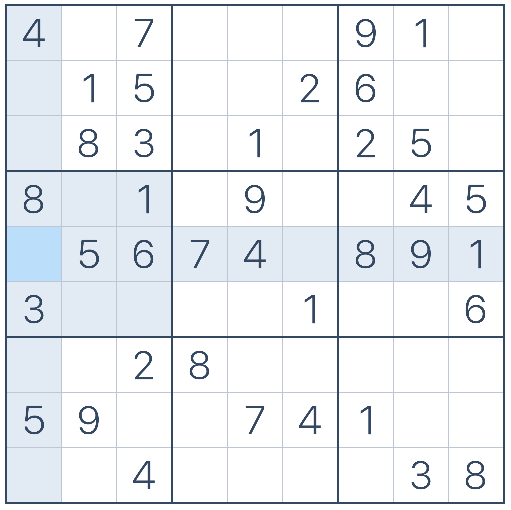
\includegraphics[width=\textwidth]{sudoku_initial_interpretation.png}
%			\end{figure}
%		\end{minipage}\hfill
%		\begin{minipage}{0.6\textwidth}
%			\begin{itemize}
%				\item[$\m{C}$] \emph{constraints} we can use to reason:
%				\begin{itemize}
%					\item alldifferent on columns (${c_1 .. c_9}$)
%					\item alldifferent on rows (${r_1 .. r_9}$)
%					\item ...
%				\end{itemize}  \pause
%				\item[$\mathcal{I}_0$] an \emph{Initial Interpretation} \pause
%				\begin{itemize}
%					\item e.g. A given Sudoku grid 
%				\end{itemize}\pause
%				\item[$\mathcal{I}_{end}$] All facts we can derive from $ \m{C} \wedge \mathcal{I}_0$ 
%				\begin{itemize}
%					\item e.g. The solution of the Sudoku grid 
%				\end{itemize}\pause
%			\end{itemize}
%		\end{minipage}		
%		
%		
%		\begin{figure}
%			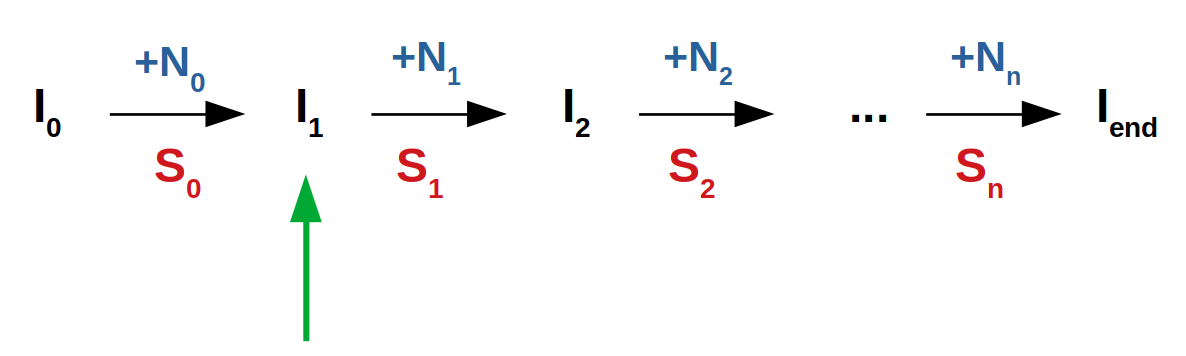
\includegraphics[width=0.7\textwidth]{sequence_explanation2.png}
%		\end{figure}
%	\end{frame}

	\begin{frame}{Explaining SAT problems}
		\framesubtitle{Non-redundant explanation}
		\begin{minipage}{0.34\textwidth}
			\begin{figure}
				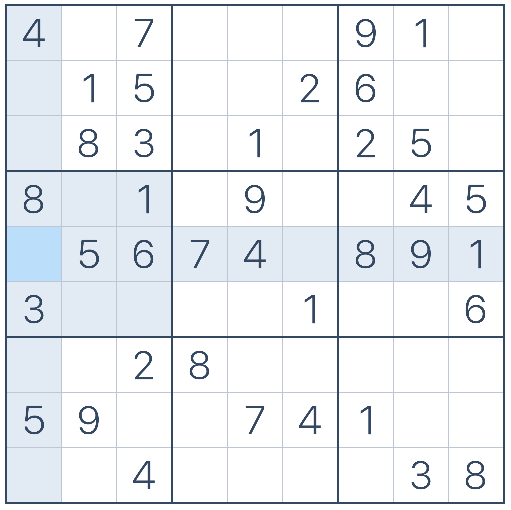
\includegraphics[width=\textwidth]{sudoku_initial_interpretation.png}
			\end{figure}
		\end{minipage}\hfill
		\begin{minipage}{0.6\textwidth}
			\begin{itemize}
				\item[$\m{C}$] \emph{constraints} we can use to reason:
				\begin{itemize}
					\item alldifferent on columns (${c_1 .. c_9}$)
					\item alldifferent on rows (${r_1 .. r_9}$)
					\item ...
				\end{itemize}  \pause
				\item[$\mathcal{I}_0$] an \emph{Initial Interpretation} \pause
				\begin{itemize}
					\item e.g. A given Sudoku grid 
				\end{itemize}\pause
				\item[$\mathcal{I}_{end}$] All facts we can propagate from $ \m{C} \wedge \mathcal{I}_0$ 
				\begin{itemize}
					\item e.g. The solution of the Sudoku grid 
				\end{itemize}
			\end{itemize}
		\end{minipage}		
		
\begin{figure}
	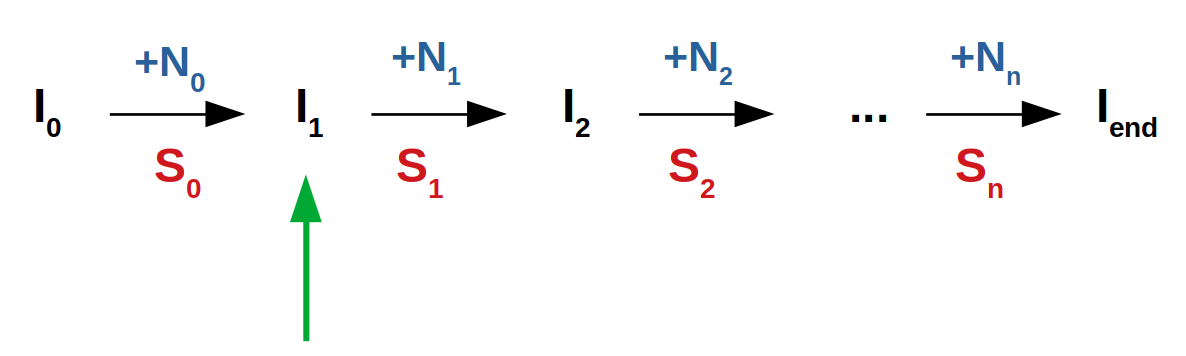
\includegraphics[width=0.7\textwidth]{sequence_explanation2.png}
\end{figure}
	
		
		
%		\begin{figure}
%			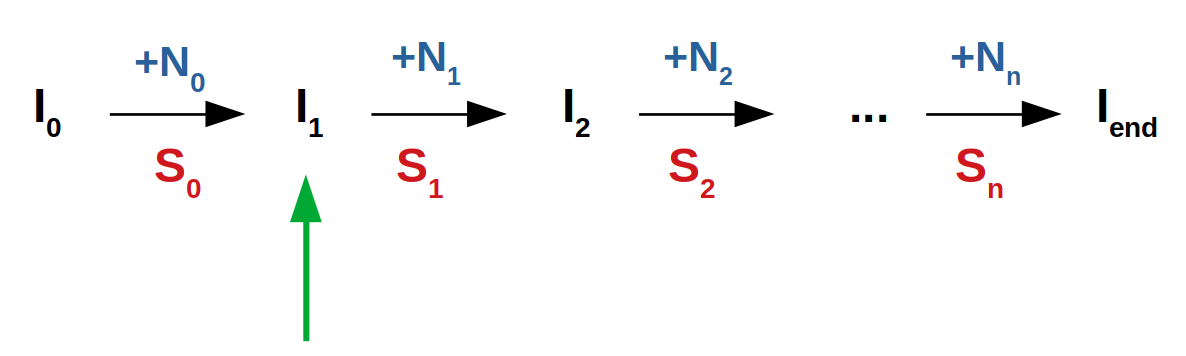
\includegraphics[width=0.7\textwidth]{sequence_explanation2.png}
%		\end{figure}
	\end{frame}
	
	\begin{frame}{Explaining SAT problems}
		\framesubtitle{Explanation sequence}
		\begin{minipage}{0.34\textwidth}
			\begin{figure}
				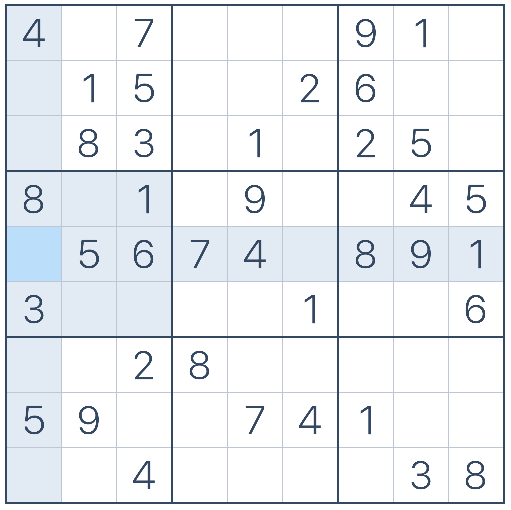
\includegraphics[width=\textwidth]{sudoku_initial_interpretation.png}
			\end{figure}
		\end{minipage}\hfill
		\begin{minipage}{0.6\textwidth}
			\begin{itemize}
				\item[$\m{C}$] \emph{constraints} we can use to reason:
				\begin{itemize}
					\item alldifferent on columns (${c_1 .. c_9}$)
					\item alldifferent on rows (${r_1 .. r_9}$)
					\item ...
				\end{itemize}  
				\item[$\mathcal{I}_0$] an \emph{Initial Interpretation} 
				\begin{itemize}
					\item e.g. A given Sudoku grid 
				\end{itemize}
				\item[$\mathcal{I}_{end}$] All facts we can propagate from $ \m{C} \wedge \mathcal{I}_0$ 
				\begin{itemize}
					\item e.g. The solution of the Sudoku grid 
				\end{itemize}
			\end{itemize}
		\end{minipage}		
		
				\begin{definition}
				Given one or a subset of the constraints ( $S_i \subseteq C$  ) and facts we know ($E_i\subseteq \mathcal{I}_i$), a non-redundant \textbf{explanation} is an implication of the form $E_i \wedge S_i  \implies N_i $, where $N_i$ is the new information from $S_i \cup E_i \models N_i$.
			\end{definition}
		
				
	\end{frame}
	
	\begin{frame}{Explaining SAT problems}
		\framesubtitle{A non-redundant explanation}
		 If we want to explain a fact $\ell \in N_i$, How can we find a non-redundant explanation? 
\begin{center}
	MUS($\formulac \land \mathcal{I} \land \neg \ell $) extraction 
\end{center}\pause
\begin{itemize}
	\item \textbf{Optimality}
	\begin{itemize}
		\item cost function quantifying the difficulty to understand the explanation, e.g. weighted sum of constraints
	\end{itemize}\pause
	\item \textbf{Constrained}:
	\begin{itemize}
		\item Additional constraints on the form of the explanation
	\end{itemize}\pause
	 \item \textbf{Incremental}
	 \begin{itemize}
	 	\item Sequence of explanations
	 	\item apply modifications and re-compute a new model?
	 \end{itemize}
\end{itemize}
\end{frame}


%	\begin{frame}{Contributions}
%		In this paper, we
%			\begin{description}[font=\color{vuborange}\itshape]
%			\item[Optimality] introduce (cost-)\textbf{\underline{O}ptimal} \underline{U}nsatisfiable \underline{S}ubsets (OUS) using the implicit hitting set duality.
%			\item[Efficiency] Add bounded and sorted OUS calls to improve time to find the next best explanation.
%			\item[Constrainedness] Analyze the structural constraint on the form of the explanations.
%			\item[Incrementality] Reuse-information between successive explanation calls to improve the efficiency of explanation sequence generation.
%		\end{description}
%		\vfill
%	\end{frame}
	
%	\begin{frame}[allowframebreaks]
%		\frametitle{References}
%		\bibliographystyle{named}
%		\bibliography{refs}
%	\end{frame}

\end{document}